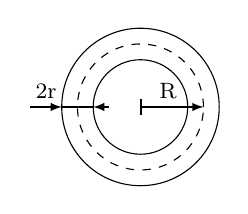
\begin{tikzpicture}
    \footnotesize
    \begin{scope}[x={(0mm,0.9\textwidth)},y={(0mm,30mm)}]
        \draw (0mm,0mm) circle[radius = 6mm];
        \draw (0mm,0mm) circle[radius = 10mm];
        \draw[dashed] (0mm,0mm) circle[radius = 8mm];
        \draw[|-latex] (0mm,0mm) -- (8mm,0mm);
        \draw (3.5mm,2mm) node {R};
        \draw[-latex] (-14mm,0mm) -- (-10mm,0mm);
        \draw (-12mm,2mm) node {2r};
        \draw (-10mm,0mm) -- (-6mm,0mm);
        \draw[latex-] (-6mm,0mm) -- (-4mm,0mm);
    \end{scope}
\end{tikzpicture}
